\documentclass[10pt]{beamer}
\usetheme{SimplePlus}
\usepackage[T1]{fontenc}
\usefonttheme[onlymath]{serif}

\usepackage{amssymb,amsmath,mathtools,stmaryrd}
\usepackage{graphicx}
\usepackage[export]{adjustbox}
\usepackage[font=scriptsize,labelfont=scriptsize]{caption}
\usepackage{tikz}
\usetikzlibrary{positioning,patterns,calc}
\graphicspath{{../Koornwinder_polynomials/}{Example of previous presentation/}{../../Talks/Interpolation_Macdonald_polynomials_ASM_session/}}

% Colors (as in the previous talk)
\definecolor{uibred}  {HTML}{db3f3d}
\definecolor{uibblue} {HTML}{4ea0b7}
\definecolor{uibgreen}{HTML}{5e8340}
\definecolor{uiblink2}{HTML}{004f6a}
\definecolor{blue}{RGB}{40,68,104}
\definecolor{slate}{HTML}{3A5A8C}
% Colour rules: \notion (green) introduces a notion or a reference; \important (red) highlights something important.
\definecolor{actblue}{RGB}{0,102,214}
\newcommand{\act}[1]{\textcolor{actblue}{#1}}
\newcommand{\qk}[1]{\alt<2->{\textcolor{uibred}{q^{#1}}}{q^{#1}}}
\newcommand{\notion}[1]{\textcolor{uibgreen}{#1}}
\newcommand{\important}[1]{\textcolor{uibred}{#1}}
\setbeamercolor{alerted text}{fg=uibred}
\setbeamerfont{frametitle}{size=\large}
\setbeamerfont{block title}{size=\normalsize}
\newcommand{\rstar}{\textcolor{uibred}{\boldsymbol{\ast}}}
\newcommand{\semitransp}[2][35]{\textcolor{fg!#1}{#2}}

% Notation of the paper
\newcommand{\ZZ}{\mathbb Z}
\newcommand{\QQ}{\mathbb Q}
\newcommand{\KK}{\mathbb K}
\newcommand{\Sign}{\mathrm{Sign}}
\newcommand{\hb}[1]{\overline{#1}}
\DeclareMathOperator{\wt}{wt}
\DeclareMathOperator{\skipped}{skip}
\DeclareMathOperator{\free}{free}
\DeclareMathOperator{\lb}{lb}
\DeclareMathOperator{\Top}{Top}
\newcommand{\conf}[2][2]{%
  \begingroup
  \renewcommand{\arraystretch}{1.25}%
  \left[
  \begin{array}{@{\;}c*{\numexpr#1-1\relax}{@{\quad}c}@{\;}}
  #2
  \end{array}
  \right]%
  \endgroup
}

% compact two-line configuration (smaller column separation)
\newcommand{\cconf}[2][2]{%
  \begingroup
  \renewcommand{\arraystretch}{1.1}%
  \left[
  \begin{array}{@{\,}c*{\numexpr#1-1\relax}{@{\;\;}c}@{\,}}
  #2
  \end{array}
  \right]%
  \endgroup
}

% Title page: SimplePlus template with a smaller top space (6em -> 2.5em)
\makeatletter
\setbeamertemplate{title page}{%
    \vspace{2.5em}
    \begingroup
    \centering
    \begin{beamercolorbox}[sep=10pt,center]{title}
        \usebeamerfont{title}\inserttitle\par%
        \ifx\insertsubtitle\@empty%
        \else%
        \vskip0.25em%
        {\usebeamerfont{subtitle}\usebeamercolor[fg]{subtitle}\insertsubtitle\par}%
        \fi%
    \end{beamercolorbox}%
    \vskip0.5em\par
    \begin{beamercolorbox}[sep=8pt,center]{author}
        \usebeamerfont{author}\insertauthor
    \end{beamercolorbox}
    \vskip-1em
    \begin{beamercolorbox}[sep=8pt,center]{institute}
        \usebeamerfont{institute}\insertinstitute
    \end{beamercolorbox}
    \begin{beamercolorbox}[sep=8pt,center]{date}
        \usebeamerfont{date}\insertdate
    \end{beamercolorbox}\vskip0.5em
    {\usebeamercolor[fg]{titlegraphic}\inserttitlegraphic\par}
    \endgroup
    \vfill
}
\makeatother

\title[Two-row recurrence for Koornwinder polynomials]{Two-row recurrence for Koornwinder polynomials}
\author[Houcine Ben Dali]{Houcine Ben Dali}
\institute{Harvard University\\[1.8em]
  {\large joint work with Lauren Williams}}
\setbeamerfont{author}{size=\large}
\setbeamerfont{institute}{size=\small}
\setbeamerfont{date}{size=\small}
\date{{\large\textcolor{uibgreen}{Conférence en l'honneur de Philippe Biane}}\\[0.4em]
  Paris, Sorbonne Université\\[0.2em]
  October 19, 2026}

\newtheorem*{prop}{Proposition}
\newtheorem*{thmA}{Theorem A}
\newtheorem*{thmB}{Theorem B}
\newtheorem*{thmC}{Theorem C}
% Multiline queues (TikZ)
\definecolor{strandA}{HTML}{159A9C}
\definecolor{strandB}{HTML}{9B1B9E}
\tikzset{
  mlqball/.style={circle,draw,inner sep=0pt,minimum size=5.5mm,font=\small,fill=white},
  mlqpt/.style={circle,fill=black,inner sep=0pt,minimum size=1.6pt},
  sA/.style={strandA,line width=0.9pt},
  sB/.style={strandB,line width=0.9pt}}
% grid: #1 = bottom y, #2 = number of rows
\newcommand{\mlqgrid}[2]{%
  \foreach \r in {1,...,#2} {
    \node[font=\small,anchor=east] at (0.3,#1+\r-1) {Row \r};
    \foreach \c in {1,...,8} \node[mlqpt] at (\c,#1+\r-1) {};}}
% bottom layer (rows 1-2) of the example, bottom row at y=#1
\newcommand{\mlqbottomlayer}[1]{%
  \draw[sB] (5,#1+1) to[out=-90,in=180] (5.5,#1+0.55) to[out=0,in=90] (6,#1);
  \draw[sA] (2,#1+1) -- (2,#1);
  \draw[sA] (4,#1+1) to[out=-90,in=180] (4.6,#1+0.45) -- (6.4,#1+0.45) to[out=0,in=90] (7,#1);
  \draw[sA] (6,#1+1) to[out=-90,in=180] (6.6,#1+0.6) -- (8.6,#1+0.6);
  \draw[sA] (0.45,#1+0.6) -- (0.6,#1+0.6) to[out=0,in=90] (1,#1);
  \foreach \c/\l in {2/2,4/2,5/4,6/2} \node[mlqball] at (\c,#1+1) {\l};
  \foreach \c/\l in {1/2,2/2,6/4,7/2,8/1} \node[mlqball] at (\c,#1) {\l};}
% Reflected two-line queue, top row (3,0,3,0,0,-2), bottom row (3,-1,0,0,-2,-3) (TikZ)
\newcommand{\RTLQ}{%
\begin{tikzpicture}[y=1.5cm]
  \foreach \r in {1,2} \foreach \c in {1,...,6} \node[mlqpt] at (\c,\r) {};
  \draw[green!50!black,line width=0.9pt,dashed] (1,2) -- (1,1);
  \draw[sB] (3,2) to[out=-90,in=180] (3.7,1.52) -- (6.25,1.52) to[out=0,in=90] (6.6,1.25) to[out=-90,in=0] (6.3,1) -- (6,1);
  \draw[blue!70!black,line width=0.9pt,dotted] (6,2) to[out=-90,in=10] (5.4,1.45) to[out=190,in=90] (5,1);
  \foreach \c/\l in {1/3,3/3,6/-2} \node[mlqball] at (\c,2) {$\l$};
  \foreach \c/\l in {1/3,2/-1,5/-2,6/-3} \node[mlqball] at (\c,1) {$\l$};
\end{tikzpicture}}
\newcommand{\MLQfour}{%
\begin{tikzpicture}
  \mlqgrid{1}{4}
  \draw[sB] (3,4) -- (3,3);
  \draw[sB] (3,3) to[out=-90,in=180] (3.6,2.55) -- (4.4,2.55) to[out=0,in=90] (5,2);
  \mlqbottomlayer{1}
  \node[mlqball] at (3,4) {4};
  \node[mlqball] at (3,3) {4};
\end{tikzpicture}}
\newcommand{\MLQfourDecomposed}{%
\begin{tikzpicture}
  % top: MLQ with 3 rows (rows 2-4, labels lowered by 1)
  \mlqgrid{4.4}{3}
  \draw[sB] (3,6.4) -- (3,5.4);
  \draw[sB] (3,5.4) to[out=-90,in=180] (3.6,4.95) -- (4.4,4.95) to[out=0,in=90] (5,4.4);
  \node[mlqball] at (3,6.4) {3};
  \node[mlqball] at (3,5.4) {3};
  \foreach \c/\l in {2/1,4/1,5/3,6/1} \node[mlqball] at (\c,4.4) {\l};
  % arrows between the two copies of row 2
  \foreach \c in {1,...,8} \draw[blue!50!black,<->,line width=1pt] (\c,2.65) -- (\c,3.75);
  % bottom: generalized two-line queue
  \mlqgrid{1}{2}
  \mlqbottomlayer{1}
  \node[font=\small,align=center,anchor=east] at (-1.3,5.4) {Multiline\\queue};
  \node[font=\small,align=center,anchor=east] at (-1.3,1.5) {Generalized\\two-line queue};
\end{tikzpicture}}
\begin{document}

\begin{frame}[plain,noframenumbering]
  \titlepage
\end{frame}

\begin{frame}[t]{Koornwinder polynomials}
Koornwinder polynomials are Laurent polynomials in $n$ variables, depending on six parameters $q,t,a,b,c,d$.
\begin{columns}[T]
\column{0.64\textwidth}
\begin{itemize}
  \item Koornwinder '92: \notion{symmetric} polynomials, indexed by partitions, introduced as multivariable orthogonal polynomials generalizing the Askey--Wilson polynomials (one variable).
  \item Sahi '99, '00: double affine Hecke algebra of type $(C^\vee,C)$, used to prove Macdonald's duality conjecture for Koornwinder polynomials and to define the \notion{nonsymmetric} Koornwinder polynomials.
  \item<3-> Cantini--Garbali--de Gier--Wheeler '16: connected Koornwinder polynomials to \important{interacting particle systems} (multispecies ASEP with open boundaries).
\end{itemize}
\column{0.33\textwidth}
\centering
\uncover<2->{%
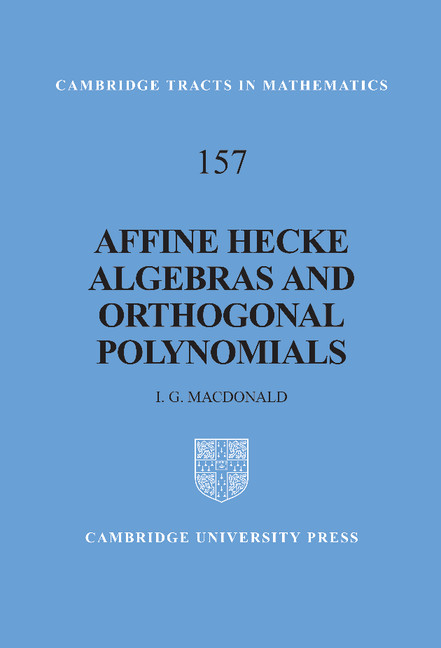
\includegraphics[height=0.4\textheight]{Book cover.jpg}\par\smallskip
Macdonald '03}
\end{columns}


\end{frame}

\begin{frame}{A family of families}
\centering
\begin{tikzpicture}[
  fam/.style={draw=uiblink2,rounded corners,line width=0.6pt,fill=uiblink2!5,align=center,inner sep=3pt,font=\footnotesize},
  arr/.style={-latex,line width=0.6pt,uiblink2},
  lab/.style={font=\scriptsize,text=black!60,align=center}]
  \node[fam] (K) at (0,0) {Koornwinder polynomials\\[1pt] {\scriptsize parameters: $q,t,a,b,c,d$}};
  \node[fam] (AW) at (-3.85,-2.3) {Askey--Wilson\\ polynomials\\[1pt] {\scriptsize parameters: $q,a,b,c,d$}};
  \node[fam] (A) at (0,-2.3) {Macdonald polynomials\\ of type $A$\\[1pt] {\scriptsize parameters: $q,t$}};
  \node[fam] (BC) at (3.85,-2.3) {Macdonald polynomials\\ of types $B$, $C$, $D$, \dots\\[1pt] {\scriptsize parameters: $q,t$,}\\[-1pt] {\scriptsize and some of $a,b,c,d$}};
  \node[fam] (J) at (-1.2,-3.95) {Jack\\[1pt] {\scriptsize parameter: $\alpha$}};
  \node[fam] (HL) at (1.2,-3.95) {Hall--Littlewood\\[1pt] {\scriptsize parameter: $t$}};
  \node[fam] (S) at (0,-5.4) {Schur, key polynomials, Demazure atoms\\[1pt] {\scriptsize no parameter}};
  \draw[arr] (K.west) -- node[lab,sloped,above] {one variable} (AW.north);
  \draw[arr] (K) -- node[lab,right=2pt] {top homogeneous\\ part {\large$\rstar$}} (A);
  \draw[arr] (K.east) -- node[lab,sloped,above] {specialization} (BC.north);
  \draw[arr] (A) -- node[lab,midway,left=3pt] {$q=t^\alpha$, $t\to1$} (J);
  \draw[arr] (A) -- node[lab,right=3pt] {$q=0$} (HL);
  \draw[arr] (J) -- node[lab,left=3pt] {$\alpha=1$} (S);
  \draw[arr] (HL) -- node[lab,right=3pt] {$t=0$} (S);
\end{tikzpicture}

\vfill
{\raggedright\scriptsize {\large$\rstar$} Symmetric case: van Diejen '95. Nonsymmetric case: BD--Williams.\par}
\end{frame}

\begin{frame}{Two nonsymmetric refinements of the symmetric Koornwinder polynomials}
\centering
\begin{tikzpicture}[
  fam/.style={draw=uiblink2,rounded corners,line width=0.6pt,fill=uiblink2!5,align=center,inner sep=3pt,font=\footnotesize},
  arr/.style={-latex,line width=0.6pt,uiblink2},
  desc/.style={align=center,font=\footnotesize,text width=3.6cm}]
  \node[fam] (K) at (0,0) {Symmetric Koornwinder polynomials\\[1pt] $K_\lambda(z_1,\dots,z_n;q,t,a,b,c,d)$};
  \node[fam] (E) at (-3.4,-1.9) {Nonsymmetric\\ Koornwinder\\ polynomials $E_\eta$};
  \node[fam] (F) at (3.4,-1.9) {Koornwinder ASEP\\ polynomials $F_\eta$};
  \draw[arr] (K) -- (E);
  \draw[arr] (K) -- (F);
  \draw[arr,latex-latex,dashed] (E) -- node[above,font=\scriptsize,text=black!60] {Kasatani '11} (F);
  \node[desc,below=6pt of E] {defined as eigenfunctions of the Cherednik operators};
  \node[desc,below=6pt of F] {defined by the $q$KZ relations};
\end{tikzpicture}

\pause
\begin{columns}[c]
\column{0.6\textwidth}
\begin{theorem}[Cantini--Garbali--de Gier--Wheeler '16]
For suitable $a,b,c,d$ depending on the boundary rates, the stationary probability of a state $\mu$ of the multispecies ASEP with open boundaries on $n$ sites is proportional to $F_\mu(\important{z_1=\dots=z_n=1};\,\important{q=1},t,a,b,c,d)$.
\end{theorem}
\column{0.38\textwidth}
\centering
\begin{tikzpicture}[x=0.58cm,y=0.58cm,
  site/.style={draw=black!40,minimum size=0.58cm,inner sep=0pt},
  ball/.style={circle,draw=uiblink2,fill=uiblink2!10,minimum size=0.5cm,inner sep=0pt,font=\scriptsize},
  hop/.style={-latex,uiblink2,line width=0.5pt},
  rl/.style={font=\scriptsize,text=black!60}]
  \foreach \i in {1,...,5} \node[site] (s\i) at (\i,0) {};
  \node[ball] at (s1) {$2$};
  \node[ball] at (s2) {$-1$};
  \node[ball] at (s4) {$1$};
  \node[ball] at (s5) {$-2$};
  \draw[hop] (s2.north) to[bend left=60] node[rl,above] {$1$} (s3.north);
  \draw[hop] (s5.south) to[bend left=60] node[rl,below] {$t$} (s4.south);
  \draw[hop] (-0.2,0.5) to[bend left=30] node[rl,above] {$\alpha$} (s1.north);
  \draw[hop] (s1.south) to[bend left=30] node[rl,below] {$\gamma$} (-0.2,-0.5);
  \draw[hop] (s5.north) to[bend left=30] node[rl,above] {$\beta$} (6.2,0.5);
  \draw[hop] (6.2,-0.5) to[bend left=30] node[rl,below] {$\delta$} (s5.south);
\end{tikzpicture}
\end{columns}
\end{frame}


\begin{frame}{Some examples of Koornwinder ASEP polynomials for $n=3$}
\scriptsize
\begin{align*}
&F_{(0,1,0)} = \important{z_2}+\frac{t\bigl(t^2ac(b+d)-a-c\bigr)}{1-t^4abcd}
\end{align*}
\pause
\vspace{-0.8em}
\begin{align*}
&F_{(0,1,-1)} = z_2z_3^{-1}+\frac{tbd(a+c)-b-d}{1-t^2abcd}\,z_2+\frac{t\bigl(tac(b+d)-a-c\bigr)}{1-t^2abcd}\,z_3^{-1}\\
&\qquad+\frac{t}{(1-t^2abcd)(1-t^3abcd)}\Bigl((a+c)(b+d)-t\bigl(ac(b+d)^2+bd(a+c)^2-abcd\bigr)\\
&\qquad\qquad+t^2abcd\bigl((a+c)(b+d)-1\bigr)-t^3(1-t)(abcd)^2\Bigr)
\end{align*}

\vfill
{\normalsize In the cases of nonnegative compositions, the top degree part is represented in \important{red}. We will see that it corresponds to type A ASEP polynomials.\par}
\end{frame}

\begin{frame}{Some examples of Koornwinder ASEP polynomials for $n=3$}
\scriptsize\setlength{\jot}{1pt}
\begin{align*}
&F_{(0,2,0)} = \important{z_2^2+\frac{1-t}{1-qt}\bigl(z_1+qz_3\bigr)z_2}+\frac{q(1-t)}{1-qt}\bigl(z_1^{-1}+z_3^{-1}\bigr)z_2+\frac{qt\bigl(qt^2ac(b+d)-a-c\bigr)}{1-q^2t^4abcd}z_2^{-1}\\
&\qquad+\frac{qt(1-t)\bigl(qt^2ac(b+d)-a-c\bigr)}{(1-qt)(1-q^2t^4abcd)}\,\bigl(z_1+q\,z_1^{-1}+z_3+z_3^{-1}\bigr)\\
&\qquad-\frac{1}{(1-qt)(1-q^2t^4abcd)}\Bigl(q^3t^5\bigl(ac(b+d)+bd(a+c)\bigr)+q^2t^4ac(b+d)-q^2t^3ac(b+d)\\
&\qquad\quad-q^2t^2bd(a+c)-q^2t^3(a+b+c+d)-qt^2ac(b+d)-qt^2(a+c)\\
&\qquad\quad+qt(a+c)+q(b+d)+a+c\Bigr)z_2\\
&\qquad-\frac{1}{(1-qt)(1-qt^4abcd)(1-q^2t^4abcd)}\Bigl(q^4t^6abcd\bigl(t^3abcd+t^2(a+c)(b+d)\\
&\qquad\qquad-t^2abcd+t^2ac+tabcd-1\bigr)\\
&\qquad\quad+q^3t^4\bigl(t^4a^2c^2(b+d)^2-t^4a^2bc^2d-t^3a^2b^2c^2d^2-t^2bd(a+c)^2-t^2ac(a+c)(b+d)\\
&\qquad\qquad-t^2ac(b+d)^2-tabcd(a+c)(b+d)+t^2abcd-ta^2bc^2d-tabcd+abcd\bigr)\\
&\qquad\quad-q^2t^2\bigl(t^4ac(a+c)(b+d)+t^3a^2c^2(b+d)^2-t^3a^2bc^2d+t^3abcd\\
&\qquad\qquad-t^2(a+c)^2-t^2(a+c)(b+d)-t^2abcd-tbd(a+c)^2-tac(a+c)(b+d)\\
&\qquad\qquad-tac(b+d)^2+t^2ac+tabcd-1\bigr)\\
&\qquad\quad+q\bigl(t^3ac(a+c)(b+d)+t^4ac+t^3abcd-t(a+c)^2-t(a+c)(b+d)\\
&\qquad\qquad-t^2+tac+t-1\bigr)-tac\Bigr)
\end{align*}
\end{frame}

\begin{frame}{Some examples of Koornwinder ASEP polynomials for $n=3$}
$F_{(0,2,1)}=$\par\smallskip
\centering
\adjustbox{max width=\textwidth, max totalheight=0.66\textheight}{%
\parbox{27cm}{\raggedright\small
$\important{z_{2}^{2}z_{3}}
\important{+\frac{(1-t)}{(1-q t^{2})}z_{1}z_{2}z_{3}}
+\frac{1}{(1-q t^{2})(1-t^{2} a b c d)(1-q^{2} t^{4} a b c d)}\bigl(q^{3} t^{8} a^{2} b^{2} c^{2} d + q^{3} t^{8} a^{2} b c^{2} d^{2} + q^{3} t^{7} a^{2} b^{2} c d^{2} + q^{3} t^{7} a b^{2} c^{2} d^{2} + q^{2} t^{7} a^{2} b^{2} c^{2} d + q^{2} t^{7} a^{2} b c^{2} d^{2} - q^{3} t^{7} a^{2} b c d - q^{3} t^{7} a b c^{2} d - q^{2} t^{6} a^{2} b^{2} c^{2} d - q^{2} t^{6} a^{2} b c^{2} d^{2} + q^{3} t^{6} a^{2} b c d + q^{3} t^{6} a b c^{2} d - q^{2} t^{6} a^{2} b c d - q^{2} t^{6} a b c^{2} d - q^{2} t^{4} a^{2} b^{2} c d^{2} - q^{2} t^{4} a b^{2} c^{2} d^{2} + q^{2} t^{5} a^{2} b c d - q^{2} t^{5} a b^{2} c d + q^{2} t^{5} a b c^{2} d - q t^{4} a^{2} b^{2} c^{2} d - q^{2} t^{5} a b c d^{2} - q t^{4} a^{2} b c^{2} d^{2} - q^{3} t^{5} a b c - q^{3} t^{5} a b d - q^{3} t^{5} a c d - q^{3} t^{5} b c d - q^{2} t^{4} a^{2} b c d - q t^{5} a^{2} b c d - q^{2} t^{4} a b c^{2} d - q t^{5} a b c^{2} d + q t^{4} a^{2} b c d + q t^{4} a b c^{2} d - q^{2} t^{4} a b c - q^{2} t^{4} a c d + q^{2} t^{3} a b c + q^{2} t^{3} a c d + q t^{2} a b^{2} c d + q t^{2} a b c d^{2} - q t^{3} a b c + q^{2} t^{2} a b d - q t^{3} a c d + q^{2} t^{2} b c d + t^{2} a^{2} b c d + t^{2} a b c^{2} d + q^{2} t^{3} a + q^{2} t^{3} b + q^{2} t^{3} c + 2 q t^{2} a b c + q^{2} t^{3} d + 2 q t^{2} a c d + q t^{3} a + q t^{3} c - q t a - q t c - q b - q d - a - c\bigr)z_{2}z_{3}
+\frac{t (t a b c + t a c d - a - c)}{(1-t^{2} a b c d)}z_{2}^{2}
+\frac{(1-t) q t ^{2} (q t^{2} a b c + q t^{2} a c d - a - c)}{(1-q t^{2})(1-q^{2} t^{4} a b c d)}z_{1}z_{3}
-\frac{t (1-t)}{(1-q t^{2})(1-t^{2} a b c d)(1-q^{2} t^{4} a b c d)}\bigl(q^{2} t^{5} a^{2} b^{2} c^{2} d + q^{2} t^{5} a^{2} b c^{2} d^{2} - q^{2} t^{5} a^{2} b c d - q^{2} t^{5} a b c^{2} d + q^{2} t^{4} a b c + q^{2} t^{4} a c d - q^{2} t^{3} a b c - q^{2} t^{3} a c d + q t^{3} a b c + q t^{3} a c d - q t^{2} a b c - q t^{2} a c d - q t^{2} a - q t^{2} c - t a b c - t a c d + q t a + q t c + a + c\bigr)z_{1}z_{2}
+\frac{(1-t) q}{(1-q t^{2})}z_{1}^{-1}z_{2}z_{3}
+\frac{1}{(1-q t^{2})(1-t^{2} a b c d)(1-q t^{3} a b c d)(1-q^{2} t^{4} a b c d)}\bigl(q^{4} t^{10} a^{3} b^{3} c^{3} d^{3} + q^{4} t^{10} a^{3} b^{3} c^{2} d^{2} + q^{4} t^{10} a^{3} b^{2} c^{3} d^{2} + q^{4} t^{10} a^{2} b^{3} c^{3} d^{2} + q^{4} t^{10} a^{3} b^{2} c^{2} d^{3} + q^{4} t^{10} a^{2} b^{2} c^{3} d^{3} + q^{3} t^{10} a^{3} b^{3} c^{3} d + q^{3} t^{10} a^{3} b^{2} c^{3} d^{2} + q^{3} t^{10} a^{3} b c^{3} d^{3} - q^{3} t^{8} a^{3} b^{3} c^{3} d^{3} + q^{3} t^{9} a^{3} b^{2} c^{3} d^{2} - q^{4} t^{9} a^{2} b^{2} c^{2} d^{2} - 2 q^{3} t^{8} a^{3} b^{2} c^{3} d^{2} - q^{3} t^{9} a^{3} b^{2} c^{2} d - q^{3} t^{9} a^{2} b^{2} c^{3} d - q^{3} t^{9} a^{3} b c^{2} d^{2} - q^{4} t^{8} a^{2} b^{2} c^{2} d^{2} - q^{3} t^{7} a^{3} b^{3} c^{2} d^{2} - q^{3} t^{9} a^{2} b c^{3} d^{2} - q^{3} t^{7} a^{2} b^{3} c^{3} d^{2} - q^{3} t^{7} a^{3} b^{2} c^{2} d^{3} - q^{3} t^{7} a^{2} b^{2} c^{3} d^{3} - q^{3} t^{8} a^{2} b^{3} c^{2} d - q^{2} t^{7} a^{3} b^{3} c^{3} d - q^{3} t^{8} a^{3} b^{2} c d^{2} - 3 q^{3} t^{8} a^{2} b^{2} c^{2} d^{2} - q^{3} t^{8} a b^{2} c^{3} d^{2} - q^{2} t^{7} a^{3} b^{2} c^{3} d^{2} - q^{3} t^{8} a^{2} b c^{2} d^{3} - q^{2} t^{7} a^{3} b c^{3} d^{3} - q^{4} t^{8} a^{2} b^{2} c d - q^{4} t^{8} a^{2} b c^{2} d - q^{4} t^{8} a b^{2} c^{2} d - q^{2} t^{8} a^{3} b^{2} c^{2} d - q^{2} t^{8} a^{2} b^{2} c^{3} d - q^{4} t^{8} a^{2} b c d^{2} - q^{4} t^{8} a b c^{2} d^{2} - q^{2} t^{8} a^{3} b c^{2} d^{2} - q^{3} t^{7} a^{2} b^{2} c^{2} d^{2} - q^{2} t^{8} a^{2} b c^{3} d^{2} + q^{3} t^{8} a^{2} b c^{2} d + 2 q^{3} t^{6} a^{2} b^{2} c^{2} d^{2} - q^{3} t^{7} a^{2} b^{2} c^{2} - 3 q^{3} t^{7} a^{2} b c^{2} d + q^{2} t^{6} a^{3} b^{2} c^{2} d + q^{2} t^{6} a^{2} b^{2} c^{3} d - q^{3} t^{7} a^{2} c^{2} d^{2} + q^{2} t^{6} a^{3} b c^{2} d^{2} - q^{2} t^{6} a^{2} b^{2} c^{2} d^{2} + q^{2} t^{6} a^{2} b c^{3} d^{2} + q^{4} t^{7} a b c d + q^{2} t^{7} a^{3} b c d + 2 q^{3} t^{6} a^{2} b c^{2} d + 2 q^{2} t^{7} a^{2} b c^{2} d + q^{2} t^{5} a^{2} b^{3} c^{2} d + q^{2} t^{7} a b c^{3} d + q^{2} t^{5} a^{3} b^{2} c d^{2} + 4 q^{2} t^{5} a^{2} b^{2} c^{2} d^{2} + q^{2} t^{5} a b^{2} c^{3} d^{2} + q^{2} t^{5} a^{2} b c^{2} d^{3} - q^{2} t^{6} a^{2} b^{2} c^{2} + q^{3} t^{5} a^{2} b^{2} c d + q^{2} t^{6} a^{2} b^{2} c d - 3 q^{2} t^{6} a^{2} b c^{2} d + q^{3} t^{5} a b^{2} c^{2} d + q^{2} t^{6} a b^{2} c^{2} d + q t^{5} a^{3} b^{2} c^{2} d + q t^{5} a^{2} b^{2} c^{3} d + q^{3} t^{5} a^{2} b c d^{2} + q^{2} t^{6} a^{2} b c d^{2} - q^{2} t^{6} a^{2} c^{2} d^{2} + q^{3} t^{5} a b c^{2} d^{2} + q^{2} t^{6} a b c^{2} d^{2} + q t^{5} a^{3} b c^{2} d^{2} + q t^{5} a^{2} b c^{3} d^{2} + q^{3} t^{6} a^{2} b c + q^{3} t^{6} a b^{2} c + q^{3} t^{6} a b c^{2} + 2 q^{2} t^{5} a^{2} b^{2} c^{2} + q^{3} t^{6} a^{2} b d + q^{3} t^{6} a^{2} c d + 3 q^{3} t^{6} a b c d + q^{3} t^{6} a c^{2} d + q^{3} t^{6} b c^{2} d + 3 q^{2} t^{5} a^{2} b c^{2} d + q t^{6} a^{2} b c^{2} d + q^{3} t^{6} a c d^{2} + 2 q^{2} t^{5} a^{2} c^{2} d^{2} + q t^{4} a^{2} b^{2} c^{2} d^{2} + q^{3} t^{5} a b c d - q t^{5} a^{2} b c^{2} d + 2 q^{2} t^{5} a^{2} b c + 2 q^{2} t^{5} a b c^{2} + 2 q^{2} t^{5} a^{2} c d - q^{3} t^{4} a b c d + q^{2} t^{5} a b c d - q t^{4} a^{3} b c d + 2 q^{2} t^{5} a c^{2} d - q t^{4} a b c^{3} d - 2 q^{2} t^{4} a^{2} b c - 2 q^{2} t^{4} a b c^{2} - 2 q^{2} t^{4} a^{2} c d + q^{2} t^{4} a b c d - q t^{3} a^{2} b^{2} c d - 2 q^{2} t^{4} a c^{2} d - q t^{3} a b^{2} c^{2} d - q t^{3} a^{2} b c d^{2} - q t^{3} a b c^{2} d^{2} + q t^{4} a^{2} b c - q^{2} t^{3} a b^{2} c + q t^{4} a b c^{2} - q^{2} t^{3} a^{2} b d + q t^{4} a^{2} c d - 4 q^{2} t^{3} a b c d - q t^{4} a b c d + q t^{4} a c^{2} d - q^{2} t^{3} b c^{2} d - t^{3} a^{2} b c^{2} d - q^{2} t^{3} a c d^{2} - q^{2} t^{4} a^{2} - q^{2} t^{4} a b - q^{2} t^{4} a c - q^{2} t^{4} b c - 2 q t^{3} a^{2} b c - q^{2} t^{4} c^{2} - 2 q t^{3} a b c^{2} - q^{2} t^{4} a d - q^{2} t^{4} c d - 2 q t^{3} a^{2} c d + q t^{3} a b c d - 2 q t^{3} a c^{2} d - q t^{4} a c - 2 q t^{2} a b c d - q t^{3} a^{2} - q t^{3} a c - q t^{3} c^{2} - q^{2} t^{3} + 2 q t^{2} a^{2} + 2 q t^{2} a c + 2 q t^{2} c^{2} + q t a b + q t b c + q t a d + q t c d + q t^{2} + t a c - q t + q\bigr)z_{3}
+\frac{1}{(1-q t^{2})(1-t^{2} a b c d)(1-q t^{3} a b c d)(1-q^{2} t^{4} a b c d)}\bigl(q^{4} t^{11} a^{3} b^{3} c^{3} d + q^{4} t^{11} a^{3} b^{2} c^{3} d^{2} + q^{4} t^{11} a^{3} b c^{3} d^{3} + q^{4} t^{10} a^{3} b^{3} c^{2} d^{2} + q^{4} t^{10} a^{3} b^{2} c^{3} d^{2} + q^{4} t^{10} a^{2} b^{3} c^{3} d^{2} + q^{4} t^{10} a^{3} b^{2} c^{2} d^{3} + q^{4} t^{10} a^{2} b^{2} c^{3} d^{3} + q^{3} t^{10} a^{3} b^{3} c^{3} d + q^{3} t^{10} a^{3} b^{2} c^{3} d^{2} + q^{3} t^{10} a^{3} b c^{3} d^{3} - q^{4} t^{10} a^{3} b^{2} c^{2} d - q^{4} t^{10} a^{2} b^{2} c^{3} d - q^{3} t^{9} a^{3} b^{3} c^{3} d - q^{4} t^{10} a^{3} b^{2} c d^{2} - q^{4} t^{10} a^{3} b c^{2} d^{2} - q^{4} t^{10} a^{2} b^{2} c^{2} d^{2} - q^{4} t^{10} a^{2} b c^{3} d^{2} - q^{4} t^{10} a b^{2} c^{3} d^{2} + q^{3} t^{9} a^{3} b^{2} c^{3} d^{2} - q^{3} t^{9} a^{3} b c^{3} d^{3} - q^{4} t^{9} a^{2} b^{2} c^{2} d^{2} - 2 q^{3} t^{8} a^{3} b^{2} c^{3} d^{2} - 2 q^{3} t^{9} a^{3} b^{2} c^{2} d - 2 q^{3} t^{9} a^{2} b^{2} c^{3} d - 2 q^{3} t^{9} a^{3} b c^{2} d^{2} - q^{3} t^{7} a^{3} b^{3} c^{2} d^{2} - 2 q^{3} t^{9} a^{2} b c^{3} d^{2} - q^{3} t^{7} a^{2} b^{3} c^{3} d^{2} - q^{3} t^{7} a^{3} b^{2} c^{2} d^{3} - q^{3} t^{7} a^{2} b^{2} c^{3} d^{3} + q^{4} t^{9} a^{2} b^{2} c d + q^{4} t^{9} a^{2} b c^{2} d + q^{4} t^{9} a b^{2} c^{2} d + q^{3} t^{8} a^{3} b^{2} c^{2} d - q^{3} t^{8} a^{2} b^{3} c^{2} d + q^{3} t^{8} a^{2} b^{2} c^{3} d - q^{2} t^{7} a^{3} b^{3} c^{3} d + q^{4} t^{9} a^{2} b c d^{2} + q^{4} t^{9} a b c^{2} d^{2} + q^{3} t^{8} a^{3} b c^{2} d^{2} - 2 q^{3} t^{8} a^{2} b^{2} c^{2} d^{2} + q^{3} t^{8} a^{2} b c^{3} d^{2} - 2 q^{2} t^{7} a^{3} b^{2} c^{3} d^{2} - q^{3} t^{8} a^{2} b c^{2} d^{3} - q^{2} t^{7} a^{3} b c^{3} d^{3} - q^{4} t^{8} a^{2} b^{2} c d - q^{4} t^{8} a^{2} b c^{2} d - q^{4} t^{8} a b^{2} c^{2} d - q^{2} t^{8} a^{3} b^{2} c^{2} d - q^{2} t^{8} a^{2} b^{2} c^{3} d - q^{4} t^{8} a^{2} b c d^{2} + q^{3} t^{7} a^{3} b^{2} c d^{2} - q^{4} t^{8} a b c^{2} d^{2} - q^{2} t^{8} a^{3} b c^{2} d^{2} + q^{3} t^{7} a^{2} b^{2} c^{2} d^{2} - q^{2} t^{8} a^{2} b c^{3} d^{2} + q^{3} t^{7} a b^{2} c^{3} d^{2} + q^{3} t^{8} a^{3} b c d + q^{3} t^{8} a^{2} b^{2} c d + 3 q^{3} t^{8} a^{2} b c^{2} d + q^{3} t^{8} a b^{2} c^{2} d + q^{2} t^{7} a^{3} b^{2} c^{2} d + q^{3} t^{8} a b c^{3} d + q^{2} t^{7} a^{2} b^{2} c^{3} d + q^{3} t^{8} a^{2} b c d^{2} + q^{3} t^{8} a b c^{2} d^{2} + q^{2} t^{7} a^{3} b c^{2} d^{2} + q^{3} t^{6} a^{2} b^{2} c^{2} d^{2} + q^{2} t^{7} a^{2} b c^{3} d^{2} - q^{3} t^{7} a^{2} b^{2} c^{2} - q^{4} t^{8} a b c d - q^{3} t^{7} a^{2} b^{2} c d - 5 q^{3} t^{7} a^{2} b c^{2} d - q^{3} t^{7} a b^{2} c^{2} d + q^{2} t^{6} a^{3} b^{2} c^{2} d + q^{2} t^{6} a^{2} b^{2} c^{3} d - q^{3} t^{7} a^{2} b c d^{2} - q^{3} t^{7} a^{2} c^{2} d^{2} - q^{3} t^{7} a b c^{2} d^{2} + q^{2} t^{6} a^{3} b c^{2} d^{2} + q^{2} t^{6} a^{2} b c^{3} d^{2} + q^{4} t^{7} a b c d + q^{2} t^{7} a^{3} b c d - q^{3} t^{6} a^{2} b^{2} c d + 2 q^{3} t^{6} a^{2} b c^{2} d + 3 q^{2} t^{7} a^{2} b c^{2} d - q^{3} t^{6} a b^{2} c^{2} d + q^{2} t^{5} a^{2} b^{3} c^{2} d + q^{2} t^{7} a b c^{3} d - q^{3} t^{6} a^{2} b c d^{2} - q^{3} t^{6} a b c^{2} d^{2} + 2 q^{2} t^{5} a^{2} b^{2} c^{2} d^{2} + q^{2} t^{5} a^{2} b c^{2} d^{3} - q^{3} t^{7} a b^{2} c - 2 q^{2} t^{6} a^{2} b^{2} c^{2} - 2 q^{3} t^{7} a b c d - q^{2} t^{6} a^{3} b c d + q^{3} t^{5} a^{2} b^{2} c d - 7 q^{2} t^{6} a^{2} b c^{2} d + q^{3} t^{5} a b^{2} c^{2} d + q t^{5} a^{3} b^{2} c^{2} d - q^{2} t^{6} a b c^{3} d + q t^{5} a^{2} b^{2} c^{3} d - q^{3} t^{7} a c d^{2} + q^{3} t^{5} a^{2} b c d^{2} - 2 q^{2} t^{6} a^{2} c^{2} d^{2} + q^{3} t^{5} a b c^{2} d^{2} + q t^{5} a^{3} b c^{2} d^{2} + q t^{5} a^{2} b c^{3} d^{2} + q^{3} t^{6} a^{2} b c + q^{3} t^{6} a b^{2} c + q^{3} t^{6} a b c^{2} + 2 q^{2} t^{5} a^{2} b^{2} c^{2} + q^{3} t^{6} a^{2} b d + q^{3} t^{6} a^{2} c d + 4 q^{3} t^{6} a b c d - q^{2} t^{5} a^{2} b^{2} c d + q^{3} t^{6} a c^{2} d + q^{3} t^{6} b c^{2} d + 4 q^{2} t^{5} a^{2} b c^{2} d + q t^{6} a^{2} b c^{2} d - q^{2} t^{5} a b^{2} c^{2} d + q^{3} t^{6} a c d^{2} - q^{2} t^{5} a^{2} b c d^{2} + 2 q^{2} t^{5} a^{2} c^{2} d^{2} - q^{2} t^{5} a b c^{2} d^{2} + q^{3} t^{5} a b c d - q^{2} t^{6} a b c d + q^{2} t^{4} a^{2} b^{2} c d - 3 q t^{5} a^{2} b c^{2} d + q^{2} t^{4} a b^{2} c^{2} d + q^{2} t^{4} a^{2} b c d^{2} + q^{2} t^{4} a b c^{2} d^{2} + 3 q^{2} t^{5} a^{2} b c + q^{2} t^{5} a b^{2} c + 3 q^{2} t^{5} a b c^{2} + q t^{4} a^{2} b^{2} c^{2} + 3 q^{2} t^{5} a^{2} c d - q^{3} t^{4} a b c d + 3 q^{2} t^{5} a b c d - q t^{4} a^{3} b c d + 3 q^{2} t^{5} a c^{2} d + 2 q t^{4} a^{2} b c^{2} d - q t^{4} a b c^{3} d + q^{2} t^{5} a c d^{2} + q t^{4} a^{2} c^{2} d^{2} - 2 q^{2} t^{4} a^{2} b c + q^{2} t^{4} a b^{2} c - 2 q^{2} t^{4} a b c^{2} - 2 q^{2} t^{4} a^{2} c d + 2 q^{2} t^{4} a b c d - 2 q^{2} t^{4} a c^{2} d + q^{2} t^{4} a c d^{2} - q^{2} t^{5} a c + 2 q t^{4} a^{2} b c - q^{2} t^{3} a b^{2} c + 2 q t^{4} a b c^{2} - q^{2} t^{3} a^{2} b d + 2 q t^{4} a^{2} c d - 4 q^{2} t^{3} a b c d + 2 q t^{4} a c^{2} d - q^{2} t^{3} b c^{2} d - q^{2} t^{3} a c d^{2} - q^{2} t^{4} a^{2} - q^{2} t^{4} a b - q^{2} t^{4} a c - q^{2} t^{4} b c - 3 q t^{3} a^{2} b c - q^{2} t^{4} c^{2} - 3 q t^{3} a b c^{2} - q^{2} t^{4} a d - q^{2} t^{4} c d - 3 q t^{3} a^{2} c d + q t^{3} a b c d - 3 q t^{3} a c^{2} d - q t^{4} a c - q t^{2} a b^{2} c - 3 q t^{2} a b c d - q t^{2} a c d^{2} + q^{2} t^{4} - 2 q t^{3} a^{2} - q t^{3} a c - t^{2} a^{2} b c - 2 q t^{3} c^{2} - t^{2} a b c^{2} - t^{2} a^{2} c d - t^{2} a c^{2} d - q^{2} t^{3} + 2 q t^{2} a^{2} + 2 q t^{2} a c + 2 q t^{2} c^{2} + q t a b + q t b c + q t a d + q t c d + t a^{2} + 2 t a c + t c^{2} - q t + q\bigr)z_{2}
-\frac{(1-t) q t ^{2}}{(1-q t^{2})(1-t^{2} a b c d)(1-q t^{3} a b c d)(1-q^{2} t^{4} a b c d)}\bigl(q^{2} t^{7} a^{3} b^{3} c^{3} d + q^{2} t^{7} a^{3} b^{2} c^{3} d^{2} + q^{2} t^{7} a^{3} b c^{3} d^{3} + q^{2} t^{6} a^{3} b^{2} c^{3} d^{2} - q^{2} t^{6} a^{3} b^{2} c^{2} d - q^{2} t^{6} a^{2} b^{2} c^{3} d - q^{2} t^{6} a^{3} b c^{2} d^{2} - q^{2} t^{6} a^{2} b c^{3} d^{2} - q t^{5} a^{3} b^{2} c^{2} d - q t^{5} a^{2} b^{2} c^{3} d - q t^{5} a^{3} b c^{2} d^{2} - q t^{5} a^{2} b c^{3} d^{2} + q^{2} t^{5} a^{2} b c^{2} d - q^{2} t^{4} a^{2} b c^{2} d + q t^{4} a^{3} b c d + 2 q t^{4} a^{2} b c^{2} d + q t^{4} a b c^{3} d - q t^{3} a^{2} b^{2} c^{2} - 2 q t^{3} a^{2} b c^{2} d - q t^{3} a^{2} c^{2} d^{2} + t^{3} a^{2} b c^{2} d - t^{2} a^{2} b c^{2} d + q t^{2} a^{2} b c + q t^{2} a b c^{2} + q t^{2} a^{2} c d + q t^{2} a c^{2} d + t a^{2} b c + t a b c^{2} + t a^{2} c d + t a c^{2} d - t a c - a^{2} - a c - c^{2}\bigr)z_{1}
+\frac{(1-t) t ^{2} q ^{2} (q t^{2} a b c + q t^{2} a c d - a - c)}{(1-q t^{2})(1-q^{2} t^{4} a b c d)}z_{1}^{-1}z_{3}
-\frac{t (1-t) q}{(1-q t^{2})(1-t^{2} a b c d)(1-q^{2} t^{4} a b c d)}\bigl(q^{2} t^{5} a^{2} b^{2} c^{2} d + q^{2} t^{5} a^{2} b c^{2} d^{2} - q^{2} t^{5} a^{2} b c d - q^{2} t^{5} a b c^{2} d + q^{2} t^{4} a b c + q^{2} t^{4} a c d - q^{2} t^{3} a b c - q^{2} t^{3} a c d + q t^{3} a b c + q t^{3} a c d - q t^{2} a b c - q t^{2} a c d - q t^{2} a - q t^{2} c - t a b c - t a c d + q t a + q t c + a + c\bigr)z_{1}^{-1}z_{2}
+\frac{t q (q t^{2} a b c + q t^{2} a c d - a - c)}{(1-q^{2} t^{4} a b c d)}z_{2}^{-1}z_{3}
-\frac{t}{(1-q t^{2})(1-t^{2} a b c d)(1-q t^{3} a b c d)(1-q^{2} t^{4} a b c d)}\bigl(q^{4} t^{9} a^{3} b^{3} c^{3} d^{2} + q^{4} t^{9} a^{3} b^{2} c^{3} d^{3} + q^{4} t^{9} a^{3} b^{3} c^{2} d + q^{4} t^{9} a^{3} b^{2} c^{3} d + q^{4} t^{9} a^{2} b^{3} c^{3} d + q^{4} t^{9} a^{3} b c^{3} d^{2} + q^{4} t^{9} a^{3} b c^{2} d^{3} + q^{4} t^{9} a^{2} b c^{3} d^{3} + q^{3} t^{9} a^{3} b^{3} c^{3} + q^{3} t^{9} a^{3} b^{2} c^{3} d + 2 q^{4} t^{8} a^{3} b^{2} c^{2} d^{2} + q^{3} t^{9} a^{3} b c^{3} d^{2} + 2 q^{4} t^{8} a^{2} b^{2} c^{3} d^{2} - q^{3} t^{7} a^{3} b^{3} c^{3} d^{2} + q^{3} t^{9} a^{3} c^{3} d^{3} - q^{3} t^{7} a^{3} b^{2} c^{3} d^{3} + q^{3} t^{8} a^{3} b^{2} c^{3} d - q^{4} t^{7} a^{3} b^{2} c^{2} d^{2} + q^{3} t^{8} a^{3} b c^{3} d^{2} - q^{4} t^{7} a^{2} b^{2} c^{3} d^{2} - q^{4} t^{8} a^{3} b^{2} c d - q^{4} t^{8} a^{3} b c^{2} d - q^{4} t^{8} a^{2} b^{2} c^{2} d - q^{4} t^{8} a^{2} b c^{3} d - q^{4} t^{8} a b^{2} c^{3} d - q^{4} t^{8} a^{3} b c d^{2} - q^{4} t^{8} a^{2} b c^{2} d^{2} + q^{3} t^{7} a^{3} b^{2} c^{2} d^{2} - q^{4} t^{8} a b c^{3} d^{2} + q^{3} t^{7} a^{2} b^{2} c^{3} d^{2} - q^{3} t^{8} a^{3} b^{2} c^{2} - q^{3} t^{8} a^{2} b^{2} c^{3} - q^{3} t^{8} a^{3} b c^{2} d - 3 q^{4} t^{7} a^{2} b^{2} c^{2} d - q^{3} t^{6} a^{3} b^{3} c^{2} d - q^{3} t^{8} a^{2} b c^{3} d - q^{3} t^{6} a^{3} b^{2} c^{3} d - q^{3} t^{6} a^{2} b^{3} c^{3} d - q^{3} t^{8} a^{3} c^{2} d^{2} - 3 q^{4} t^{7} a^{2} b c^{2} d^{2} - 2 q^{3} t^{6} a^{3} b^{2} c^{2} d^{2} - q^{3} t^{8} a^{2} c^{3} d^{2} - q^{3} t^{6} a^{3} b c^{3} d^{2} - 2 q^{3} t^{6} a^{2} b^{2} c^{3} d^{2} - q^{3} t^{6} a^{3} b c^{2} d^{3} - q^{3} t^{6} a^{2} b c^{3} d^{3} - q^{3} t^{7} a^{3} b^{2} c^{2} - q^{3} t^{7} a^{2} b^{3} c^{2} - q^{3} t^{7} a^{2} b^{2} c^{3} - q^{2} t^{6} a^{3} b^{3} c^{3} - q^{3} t^{7} a^{3} b^{2} c d - 2 q^{3} t^{7} a^{3} b c^{2} d + q^{4} t^{6} a^{2} b^{2} c^{2} d - 2 q^{3} t^{7} a^{2} b^{2} c^{2} d - 2 q^{3} t^{7} a^{2} b c^{3} d - q^{3} t^{7} a b^{2} c^{3} d - q^{2} t^{6} a^{3} b^{2} c^{3} d - q^{3} t^{7} a^{3} b c d^{2} - q^{3} t^{7} a^{3} c^{2} d^{2} + q^{4} t^{6} a^{2} b c^{2} d^{2} - 2 q^{3} t^{7} a^{2} b c^{2} d^{2} - q^{3} t^{7} a^{2} c^{3} d^{2} - q^{3} t^{7} a b c^{3} d^{2} - q^{2} t^{6} a^{3} b c^{3} d^{2} - q^{3} t^{7} a^{2} c^{2} d^{3} - q^{2} t^{6} a^{3} c^{3} d^{3} - q^{2} t^{7} a^{3} b^{2} c^{2} - q^{2} t^{7} a^{2} b^{2} c^{3} + q^{4} t^{7} a^{2} b c d + q^{4} t^{7} a b c^{2} d - q^{2} t^{7} a^{3} b c^{2} d - 5 q^{3} t^{6} a^{2} b^{2} c^{2} d - q^{2} t^{7} a^{2} b c^{3} d - q^{2} t^{5} a^{3} b^{2} c^{3} d - q^{2} t^{7} a^{3} c^{2} d^{2} - 5 q^{3} t^{6} a^{2} b c^{2} d^{2} - q^{2} t^{7} a^{2} c^{3} d^{2} - q^{2} t^{5} a^{3} b c^{3} d^{2} + q^{3} t^{7} a^{2} b c^{2} + q^{3} t^{5} a^{3} b^{2} c d + q^{3} t^{7} a^{2} c^{2} d + q^{3} t^{5} a^{3} b c^{2} d - q^{2} t^{6} a^{3} b c^{2} d + 5 q^{3} t^{5} a^{2} b^{2} c^{2} d + q^{3} t^{5} a^{2} b c^{3} d - q^{2} t^{6} a^{2} b c^{3} d + q^{3} t^{5} a b^{2} c^{3} d + q^{3} t^{5} a^{3} b c d^{2} + 5 q^{3} t^{5} a^{2} b c^{2} d^{2} + q^{3} t^{5} a b c^{3} d^{2} + q^{3} t^{6} a^{3} b c + q^{3} t^{6} a^{2} b^{2} c + q^{3} t^{6} a^{2} b c^{2} + q^{3} t^{6} a b^{2} c^{2} + q^{2} t^{5} a^{3} b^{2} c^{2} + q^{3} t^{6} a b c^{3} + q^{2} t^{5} a^{2} b^{2} c^{3} + q^{3} t^{6} a^{3} b d + q^{3} t^{6} a^{3} c d + 4 q^{3} t^{6} a^{2} b c d + q^{3} t^{6} a^{2} c^{2} d + 4 q^{3} t^{6} a b c^{2} d + q^{2} t^{5} a^{3} b c^{2} d - 2 q^{2} t^{5} a^{2} b^{2} c^{2} d + q^{3} t^{6} a c^{3} d + q^{3} t^{6} b c^{3} d + q^{2} t^{5} a^{2} b c^{3} d + q^{3} t^{6} a^{2} c d^{2} + q^{3} t^{6} a c^{2} d^{2} + q^{2} t^{5} a^{3} c^{2} d^{2} - 2 q^{2} t^{5} a^{2} b c^{2} d^{2} + q^{2} t^{5} a^{2} c^{3} d^{2} + q^{2} t^{6} a^{3} b c + 2 q^{2} t^{6} a^{2} b c^{2} + q^{2} t^{4} a^{3} b^{2} c^{2} + q^{2} t^{4} a^{2} b^{3} c^{2} + q^{2} t^{6} a b c^{3} + q^{2} t^{4} a^{2} b^{2} c^{3} + q^{2} t^{6} a^{3} c d + q^{3} t^{5} a^{2} b c d + q^{2} t^{4} a^{3} b^{2} c d + 2 q^{2} t^{6} a^{2} c^{2} d + q^{3} t^{5} a b c^{2} d + 2 q^{2} t^{4} a^{3} b c^{2} d + 6 q^{2} t^{4} a^{2} b^{2} c^{2} d + q^{2} t^{6} a c^{3} d + 2 q^{2} t^{4} a^{2} b c^{3} d + q^{2} t^{4} a b^{2} c^{3} d + q^{2} t^{4} a^{3} b c d^{2} + q^{2} t^{4} a^{3} c^{2} d^{2} + 6 q^{2} t^{4} a^{2} b c^{2} d^{2} + q^{2} t^{4} a^{2} c^{3} d^{2} + q^{2} t^{4} a b c^{3} d^{2} + q^{2} t^{4} a^{2} c^{2} d^{3} + q^{2} t^{5} a^{3} b c + q^{2} t^{5} a^{2} b^{2} c + q^{2} t^{5} a^{2} b c^{2} + q^{2} t^{5} a b^{2} c^{2} + q t^{4} a^{3} b^{2} c^{2} + q^{2} t^{5} a b c^{3} + q t^{4} a^{2} b^{2} c^{3} + q^{2} t^{5} a^{3} c d - q^{3} t^{4} a^{2} b c d + 2 q^{2} t^{5} a^{2} b c d + q^{2} t^{5} a^{2} c^{2} d - q^{3} t^{4} a b c^{2} d + 2 q^{2} t^{5} a b c^{2} d + q t^{4} a^{3} b c^{2} d + q^{2} t^{5} a c^{3} d + q t^{4} a^{2} b c^{3} d + q^{2} t^{5} a^{2} c d^{2} + q^{2} t^{5} a c^{2} d^{2} + q t^{4} a^{3} c^{2} d^{2} + q t^{4} a^{2} c^{3} d^{2} - 2 q^{3} t^{5} a b c - q^{2} t^{4} a^{2} b c^{2} + q t^{5} a^{2} b c^{2} - 2 q^{3} t^{5} a c d + q^{2} t^{4} a^{2} b c d - q^{2} t^{4} a^{2} c^{2} d + q t^{5} a^{2} c^{2} d + q^{2} t^{4} a b c^{2} d + q t^{3} a^{3} b c^{2} d + q t^{3} a^{2} b^{2} c^{2} d + q t^{3} a^{2} b c^{3} d + q t^{3} a^{2} b c^{2} d^{2} - q^{2} t^{5} a^{2} c + 3 q^{3} t^{4} a b c - q^{2} t^{3} a^{3} b c - q^{2} t^{3} a^{2} b^{2} c - q^{2} t^{5} a c^{2} - q^{2} t^{3} a^{2} b c^{2} - q^{2} t^{3} a b^{2} c^{2} - q^{2} t^{3} a b c^{3} - q^{2} t^{3} a^{3} b d + 3 q^{3} t^{4} a c d - q^{2} t^{3} a^{3} c d - 5 q^{2} t^{3} a^{2} b c d - q^{2} t^{3} a^{2} c^{2} d - 5 q^{2} t^{3} a b c^{2} d - q^{2} t^{3} a c^{3} d - q^{2} t^{3} b c^{3} d - q^{2} t^{3} a^{2} c d^{2} - q^{2} t^{3} a c^{2} d^{2} - q^{2} t^{4} a^{3} - q^{2} t^{4} a^{2} b - q^{2} t^{4} a^{2} c - q^{3} t^{3} a b c - 3 q^{2} t^{4} a b c - q t^{3} a^{3} b c - q^{2} t^{4} a c^{2} - q^{2} t^{4} b c^{2} - 2 q t^{3} a^{2} b c^{2} - q^{2} t^{4} c^{3} - q t^{3} a b c^{3} - q^{2} t^{4} a^{2} d - q^{3} t^{3} a c d - 3 q^{2} t^{4} a c d - q t^{3} a^{3} c d - q^{2} t^{4} c^{2} d - 2 q t^{3} a^{2} c^{2} d - q t^{3} a c^{3} d - q t^{4} a^{2} c + 4 q^{2} t^{3} a b c - q t^{2} a^{3} b c - q t^{2} a^{2} b^{2} c - q t^{4} a c^{2} - q t^{2} a^{2} b c^{2} - q t^{2} a b^{2} c^{2} - q t^{2} a b c^{3} + 4 q^{2} t^{3} a c d - q t^{2} a^{3} c d - 3 q t^{2} a^{2} b c d - q t^{2} a^{2} c^{2} d - 3 q t^{2} a b c^{2} d - q t^{2} a c^{3} d - q t^{2} a^{2} c d^{2} - q t^{2} a c^{2} d^{2} - 2 q^{2} t^{2} a b c - q t^{3} a b c - t^{2} a^{2} b c^{2} - 2 q^{2} t^{2} a c d - q t^{3} a c d - t^{2} a^{2} c^{2} d + q^{2} t^{3} a + q^{2} t^{3} c + q t^{2} a^{2} c + 2 q t^{2} a b c + q t^{2} a c^{2} + 2 q t^{2} a c d - 3 q^{2} t^{2} a + q t a^{3} + q t a^{2} b - 3 q^{2} t^{2} c + q t a^{2} c + q t a c^{2} + q t b c^{2} + q t c^{3} + q t a^{2} d + q t c^{2} d + q^{2} t a + q t^{2} a + q^{2} t c + q t^{2} c + t a^{2} c + t a c^{2} - 2 q t a - 2 q t c + 2 q a + 2 q c\bigr)
-\frac{t (1-t) q (q t^{3} a^{2} b c d + q t^{3} a b c^{2} d - q t^{2} a b c - q t^{2} a c d - t a b c - t a c d + a + c)}{(1-t^{2} a b c d)(1-q^{2} t^{4} a b c d)}z_{2}z_{3}^{-1}
-\frac{(1-t) t ^{2} q ^{2}}{(1-q t^{2})(1-t^{2} a b c d)(1-q t^{3} a b c d)(1-q^{2} t^{4} a b c d)}\bigl(q^{2} t^{7} a^{3} b^{3} c^{3} d + q^{2} t^{7} a^{3} b^{2} c^{3} d^{2} + q^{2} t^{7} a^{3} b c^{3} d^{3} + q^{2} t^{6} a^{3} b^{2} c^{3} d^{2} - q^{2} t^{6} a^{3} b^{2} c^{2} d - q^{2} t^{6} a^{2} b^{2} c^{3} d - q^{2} t^{6} a^{3} b c^{2} d^{2} - q^{2} t^{6} a^{2} b c^{3} d^{2} - q t^{5} a^{3} b^{2} c^{2} d - q t^{5} a^{2} b^{2} c^{3} d - q t^{5} a^{3} b c^{2} d^{2} - q t^{5} a^{2} b c^{3} d^{2} + q^{2} t^{5} a^{2} b c^{2} d - q^{2} t^{4} a^{2} b c^{2} d + q t^{4} a^{3} b c d + 2 q t^{4} a^{2} b c^{2} d + q t^{4} a b c^{3} d - q t^{3} a^{2} b^{2} c^{2} - 2 q t^{3} a^{2} b c^{2} d - q t^{3} a^{2} c^{2} d^{2} + t^{3} a^{2} b c^{2} d - t^{2} a^{2} b c^{2} d + q t^{2} a^{2} b c + q t^{2} a b c^{2} + q t^{2} a^{2} c d + q t^{2} a c^{2} d + t a^{2} b c + t a b c^{2} + t a^{2} c d + t a c^{2} d - t a c - a^{2} - a c - c^{2}\bigr)z_{1}^{-1}
+\frac{q t ^{2} (t a b c + t a c d - a - c) (q t^{2} a b c + q t^{2} a c d - a - c)}{(1-t^{2} a b c d)(1-q^{2} t^{4} a b c d)}z_{2}^{-1}
-\frac{(1-t) q t ^{2}}{(1-t^{2} a b c d)(1-q t^{3} a b c d)(1-q^{2} t^{4} a b c d)}\bigl(q^{2} t^{6} a^{3} b^{2} c^{3} d^{2} - q^{2} t^{4} a^{2} b c^{2} d - q t^{3} a^{2} b^{2} c^{2} - 2 q t^{3} a^{2} b c^{2} d - q t^{3} a^{2} c^{2} d^{2} - t^{2} a^{2} b c^{2} d + q t^{2} a^{2} b c + q t^{2} a b c^{2} + q t^{2} a^{2} c d + q t^{2} a c^{2} d + t a^{2} b c + t a b c^{2} + t a^{2} c d + t a c^{2} d - a^{2} - a c - c^{2}\bigr)z_{3}^{-1}$}}
\end{frame}


\begin{frame}{The affine Weyl group of type $\widetilde C_n$}
The affine Weyl group $W$ of type $\widetilde C_n$ is generated by $s_0,s_1,\dots,s_n$ with relations
\begin{align*}
s_is_j&=s_js_i, && |i-j|\ge 2,\\
s_is_{i+1}s_i&=s_{i+1}s_is_{i+1}, && 1\le i<n-1,\\
s_0s_1s_0s_1&=s_1s_0s_1s_0,\\
s_{n-1}s_ns_{n-1}s_n&=s_ns_{n-1}s_ns_{n-1},\\
s_i^2&=1, && 0\le i\le n.
\end{align*}
\begin{center}
\begin{tikzpicture}[x=1.2cm,
  dot/.style={circle,inner sep=0pt,draw=blue,fill=white,line width=0.9pt,minimum size=6pt},
  edge/.style={line width=0.5pt}]
  \draw[edge,double distance=1.6pt] (0,0)--(1,0);
  \draw[edge] (0.423,0.11)--(0.577,0)--(0.423,-0.11);
  \draw[edge] (1,0)--(2.45,0);
  \draw[edge,dotted] (2.6,0)--(3.4,0);
  \draw[edge] (3.55,0)--(5,0);
  \draw[edge,double distance=1.6pt] (5,0)--(6,0);
  \draw[edge] (5.577,0.11)--(5.423,0)--(5.577,-0.11);
  \foreach \x/\l in {0/0,1/1,2/2,4/n-2,5/n-1,6/n}
    \node[dot,label={[label distance=1pt]below:{\small$\strut\l$}}] at (\x,0) {};
\end{tikzpicture}
\end{center}
The finite Weyl group $W_0=\langle s_1,\dots,s_n\rangle\simeq S_n\ltimes(\ZZ/2\ZZ)^n$ is the group of signed permutations.
\end{frame}

\begin{frame}{The affine Weyl group of type $\widetilde C_n$}
\begin{center}
\begin{tikzpicture}[x=1.2cm,
  dot/.style={circle,inner sep=0pt,draw=blue,fill=white,line width=0.9pt,minimum size=6pt},
  edge/.style={line width=0.5pt}]
  \draw[edge,double distance=1.6pt] (0,0)--(1,0);
  \draw[edge] (0.423,0.11)--(0.577,0)--(0.423,-0.11);
  \draw[edge] (1,0)--(2.45,0);
  \draw[edge,dotted] (2.6,0)--(3.4,0);
  \draw[edge] (3.55,0)--(5,0);
  \draw[edge,double distance=1.6pt] (5,0)--(6,0);
  \draw[edge] (5.577,0.11)--(5.423,0)--(5.577,-0.11);
  \foreach \x/\l in {0/0,1/1,2/2,4/n-2,5/n-1,6/n}
    \node[dot,label={[label distance=1pt]below:{\small$\strut\l$}}] at (\x,0) {};
\end{tikzpicture}
\end{center}
$W$ acts on Laurent polynomials in $z_1,\dots,z_n$ by
\begin{align*}
s_i(z_1,\dots,z_i,z_{i+1},\dots,z_n)
  &= (z_1,\dots,z_{i+1},z_i,\dots,z_n), && 1\le i<n,\\
s_n(z_1,\dots,z_{n-1},z_n)
  &= (z_1,\dots,z_{n-1},z_n^{-1}),\\
s_0(z_1,z_2,\dots,z_n)
  &= (\important{q}z_1^{-1},z_2,\dots,z_n).
\end{align*}
\pause
A Laurent polynomial is symmetric if it is invariant under the action of $W_0$.

\begin{exampleblock}{Example: The symmetric Koornwinder polynomial $K_{(2,0)}$}
\vspace{-1.2em}
\begin{multline*}
K_{(2,0)}=z_1^2+z_1^{-2}+z_2^2+z_2^{-2}+\frac{(1+q)(1-t)}{1-qt}\,(z_1+z_1^{-1})(z_2+z_2^{-1})\\
-\frac{(1+q)(1-qt^2)}{(1-qt)(1-q^2t^2abcd)}\big(a+b+c+d-qt(abc+abd+acd+bcd)\big)\\
\times(z_1+z_1^{-1}+z_2+z_2^{-1})+\text{constant}.
\end{multline*}
\end{exampleblock}
\end{frame}

\begin{frame}{The affine Hecke algebra $\mathcal H$ of type $\widetilde C_n$}
The affine Hecke algebra $\mathcal H$ is generated by $T_0,T_1,\dots,T_n$, subject to the braid relations
\begin{align*}
T_iT_j&=T_jT_i, && |i-j|\ge 2,\\
T_iT_{i+1}T_i&=T_{i+1}T_iT_{i+1}, && 1\le i<n-1,\\
T_0T_1T_0T_1&=T_1T_0T_1T_0,\\
T_{n-1}T_nT_{n-1}T_n&=T_nT_{n-1}T_nT_{n-1},
\end{align*}
and the quadratic relations
\[
(T_i-t_i)(T_i+1)=0,\qquad 0\le i\le n,
\]
where $\important{t_0=-ac/q}$, $\important{t_i=t}$ for $1\le i<n$, and $\important{t_n=-bd}$.
\begin{center}
\begin{tikzpicture}[x=1.2cm,
  dot/.style={circle,inner sep=0pt,draw=blue,fill=white,line width=0.9pt,minimum size=6pt},
  edge/.style={line width=0.5pt}]
  \draw[edge,double distance=1.6pt] (0,0)--(1,0);
  \draw[edge] (0.423,0.11)--(0.577,0)--(0.423,-0.11);
  \draw[edge] (1,0)--(2.45,0);
  \draw[edge,dotted] (2.6,0)--(3.4,0);
  \draw[edge] (3.55,0)--(5,0);
  \draw[edge,double distance=1.6pt] (5,0)--(6,0);
  \draw[edge] (5.577,0.11)--(5.423,0)--(5.577,-0.11);
  \foreach \x/\l/\p in {0/0/t_0,1/1/t,2/2/t,4/n-2/t,5/n-1/t,6/n/t_n}
    \node[dot,label={[label distance=1pt]below:{\small$\strut\l$}},label={[label distance=1pt]above:{$\important{\p}$}}] at (\x,0) {};
\end{tikzpicture}
\end{center}
When $t_i=1$ for all $0\le i\le n$, we get back the affine Weyl group $W$, where $T_i$ corresponds to $s_i$.
\end{frame}

\begin{frame}{Polynomial representation of $\mathcal H$}
The affine Hecke algebra $\mathcal H$ acts on Laurent polynomials in $z_1,\dots,z_n$ by the Demazure--Lusztig operators
\begin{align*}
T_i &= t + \frac{t z_i-z_{i+1}}{z_i-z_{i+1}}\,(s_i-1),
&& 1\le i<n,\\
T_n &= -bd + \frac{(1-b z_n)(1-d z_n)}{1-z_n^2}\,(s_n-1),\\
T_0 &= -\frac{ac}{q} + \frac{(1-a/z_1)(1-c/z_1)}{1-q/z_1^2}\,(s_0-1).
\end{align*}

\begin{theorem}[Sahi '99]
This representation is faithful.
\end{theorem}
% Oral remark: as a consequence, we don't lose anything by thinking of $\mathcal H$ just through these expressions.
\end{frame}

\begin{frame}{Koornwinder ASEP polynomials}
Fix a partition $\lambda$. The Koornwinder ASEP polynomials $\{F_\eta\}_{\eta\in W_0\cdot\lambda}$ are the unique family of Laurent polynomials, normalized by $[z^\eta]F_\eta=1$, satisfying the $q$KZ relations (Kasatani '11)
\begin{align*}
T_0 F_{\eta_1,\eta_2,\dots,\eta_n}&=q^{\eta_1}F_{\important{-\eta_1},\eta_2,\dots,\eta_n}, && \eta_1<0,\\
T_0 F_{\eta_1,\eta_2,\dots,\eta_n}&=t_0\,F_{\eta_1,\eta_2,\dots,\eta_n}, && \eta_1=0,\\
T_i F_{\dots,\eta_i,\eta_{i+1},\dots}&=t\,F_{\dots,\eta_i,\eta_{i+1},\dots}, && \eta_i=\eta_{i+1},\ 1\le i<n,\\
T_i F_{\dots,\eta_i,\eta_{i+1},\dots}&=F_{\dots,\important{\eta_{i+1},\eta_i},\dots}, && \eta_i>\eta_{i+1},\ 1\le i<n,\\
T_n F_{\dots,\eta_n}&=t_n\,F_{\dots,\eta_n}, && \eta_n=0,\\
T_n F_{\dots,\eta_n}&=F_{\dots,\important{-\eta_n}}, && \eta_n>0.
\end{align*}
Recall that $t_0=-ac/q$ and $t_n=-bd$.
\end{frame}

\begin{frame}{Branching rules for Schur polynomials}
\[
s_\lambda(z_1,\dots,z_n)=\sum_{\substack{\mu\subseteq\lambda\\ \lambda/\mu\text{ horizontal strip}}} z_n^{|\lambda|-|\mu|}\,s_\mu(z_1,\dots,z_{n-1}).
\]
\begin{columns}[c]
\begin{column}{0.4\textwidth}
\centering
\begin{tikzpicture}[scale=0.45]
  \foreach \r/\l in {0/3,1/2,2/1}
    \foreach \c in {1,...,\l}
      \draw[fill=black!12] (\c-1,\r) rectangle (\c,\r+1);
  \foreach \c/\r in {4/0,5/0,2/2}
    \draw[fill=uibred!35] (\c-1,\r) rectangle (\c,\r+1);
\end{tikzpicture}

\smallskip
{\small $\lambda=(5,2,2)$, $\mu=(3,2,1)$}
\end{column}
\begin{column}{0.56\textwidth}
$\lambda/\mu$ is a horizontal strip: at most one box in each column.
\end{column}
\end{columns}

% \medskip
% \begin{itemize}
%   \item Symmetric functions: equivalent to the Pieri rule $s_\mu h_k=\sum_{\lambda} s_\lambda$, over horizontal strips $\lambda/\mu$ of size $k$.
%   \item Representation theory: restriction of irreducible representations from $GL_n$ to $GL_{n-1}$ (Gelfand--Tsetlin '50).
%   \item Iterating gives the combinatorial formula $s_\lambda=\sum_T z^T$ over semistandard tableaux (Gelfand--Tsetlin patterns).
% \end{itemize}
\end{frame}

\begin{frame}{Branching rules for Macdonald polynomials}
\[
P_\lambda(z_1,\dots,z_n;q,t)=\sum_{\substack{\mu\subseteq\lambda\\ \lambda/\mu\text{ horizontal strip}}}\important{\psi_{\lambda/\mu}(q,t)}\,z_n^{|\lambda|-|\mu|}P_\mu(z_1,\dots,z_{n-1};q,t),
\]
{\small with branching coefficients (Macdonald '95)
\[
\important{\psi_{\lambda/\mu}(q,t)}=\prod_{s\in R_{\lambda/\mu}\setminus C_{\lambda/\mu}}\frac{b_\mu(s)}{b_\lambda(s)},
\qquad
b_\lambda(s)=\frac{1-q^{a_\lambda(s)}t^{l_\lambda(s)+1}}{1-q^{a_\lambda(s)+1}t^{l_\lambda(s)}},
\]
where $R_{\lambda/\mu}$ (resp.\ $C_{\lambda/\mu}$) is the union of rows (resp.\ columns) meeting $\lambda/\mu$.\par}

\pause
\medskip
Branching rules also exist for
\begin{itemize}
  \item interpolation Macdonald polynomials (Okounkov '98),
  \item symmetric Koornwinder polynomials (van Diejen--Emsiz '15).
\end{itemize}

\pause
\smallskip
These branching rules have two limitations:
\begin{itemize}
  \item they do not have a direct analogue for nonsymmetric polynomials;
  \item except for the Schur case, the branching coefficients are complicated rational expressions in $q$ and $t$, and the resulting formulas do not make integrality and positivity manifest.
\end{itemize}
\end{frame}

\begin{frame}{Type A: multiline queues}
\begin{center}
\resizebox{0.62\textwidth}{!}{\MLQfour}

{\small A multiline queue (MLQ) with $4$ rows, of type $(2,2,0,0,0,4,2,1)$.}
\end{center}
\begin{itemize}
  \item The type of an MLQ is given by the labels of its bottom row ($0$ for an empty position).
  \item Ball weight: each ball in column $i$ contributes $z_i$; here $z_1z_2^2z_3^2z_4z_5z_6^2z_7z_8$.
  \item Pairing weight: a rational function in $q,t$, multiplicative over the layers: here $\mathrm{wt}_{\mathrm{pairing}}=\mathrm{wt}_1\,\mathrm{wt}_2\,\mathrm{wt}_3$.
\end{itemize}
\begin{theorem}[Corteel--Mandelshtam--Williams '22]
For $\kappa\in\ZZ_{\ge0}^n$, $F^A_\kappa$ is the generating function of MLQs of type $\kappa$.
\end{theorem}
\end{frame}

\begin{frame}{Type A two-row recurrence}
\begin{center}
\hspace*{-0.5cm}\adjustbox{width=0.4\textwidth,valign=c}{\MLQfour}
$\equiv$
\adjustbox{width=0.55\textwidth,valign=c}{\MLQfourDecomposed}
\end{center}
Since the pairing weight is multiplicative over layers, removing the bottom layer gives
\[
F^A_\kappa(z_1,\dots,z_n;q,t)=\prod_{i:\,\kappa_i>0}z_i\sum_{\mu\in S_n\cdot\kappa^-}c^\mu_\kappa(q,t)\,F^A_\mu(z_1,\dots,z_n;q,t),
\]
where $\kappa^-_i=\max\{\kappa_i-1,0\}$, and $c^\mu_\kappa(q,t)$ is the generating function of generalized two-line queues.
\end{frame}

\begin{frame}{Type A two-row recurrence}
\begin{center}
\adjustbox{width=0.45\textwidth}{\MLQfour}
\end{center}
\vspace{0.4em}
\[
F^A_\kappa(z_1,\dots,z_n;q,t)=\prod_{i:\,\kappa_i>0}z_i\sum_{\mu\in S_n\cdot\kappa^-}c^\mu_\kappa(q,t)\,F^A_\mu(z_1,\dots,z_n;q,t)
\]
\begin{center}
\adjustbox{max width=\textwidth}{%
\begin{tikzpicture}[scale=0.4]
  % kappa
  \draw[line width=0.8pt] (0,0) -- (8,0);
  \foreach \c/\h in {1/2,2/2,6/4,7/2,8/1}
    \foreach \r in {1,...,\h}
      \draw[fill=black!12] (\c-1,\r-1) rectangle (\c,\r);
  \foreach \c in {1,2,6,7,8}
    \draw[fill=uibred!35] (\c-1,0) rectangle (\c,1);
  \foreach \c in {1,2,6,7,8}
    \node<2->[font=\footnotesize] at (\c-0.5,0.5) {$z_{\c}$};
  \node[anchor=north] at (4,-0.3) {$\kappa=(2,2,0,0,0,4,2,1)$};
  % kappa^-
  \begin{scope}[shift={(12.5,0)}]
  \uncover<3->{
  \draw[->,line width=0.8pt] (-3.5,1.5) -- (-1,1.5);
  \draw[line width=0.8pt] (0,0) -- (8,0);
  \foreach \c/\h in {1/1,2/1,6/3,7/1}
    \foreach \r in {1,...,\h}
      \draw[fill=black!12] (\c-1,\r-1) rectangle (\c,\r);
  \node[anchor=north] at (4,-0.3) {$\kappa^-=(1,1,0,0,0,3,1,0)$};}
  \end{scope}
  % mu
  \begin{scope}[shift={(25,0)}]
  \uncover<4->{
  \draw[->,line width=0.8pt] (-3.5,1.5) -- (-1,1.5);
  \node[align=center,font=\footnotesize] at (-2.25,3.4) {permute in all\\ possible ways};
  \draw[line width=0.8pt] (0,0) -- (8,0);
  \foreach \c/\h in {2/1,4/1,5/3,6/1}
    \foreach \r in {1,...,\h}
      \draw[fill=black!12] (\c-1,\r-1) rectangle (\c,\r);
  \node at (9.2,0.8) {$\cdots$};
  \node[anchor=north] at (4,-0.3) {$\mu=(0,1,0,1,3,1,0,0)$};}
  \end{scope}
\end{tikzpicture}}
\end{center}
\end{frame}

\begin{frame}{Two-row recurrence for Koornwinder polynomials}
\begin{thmA}[two-row recurrence]
For $\kappa\in\ZZ^n$, set $(\kappa^-)_i=\kappa_i-\Sign(\kappa_i)$. Then
\[
F_\kappa(z_1,\dots,z_n;q,t,a,b,c,d)=\sum_{(\nu,\mu)}a_\kappa^\mu(\nu)\,z^\nu F_\mu(z_1,\dots,z_n;q,t,a,b,c,d),
\]
where $\mu\in W_0\cdot\kappa^-$ and $\nu\in\ZZ^n$ with $\nu_i\in\{0,\Sign(\kappa_i)\}$.
\end{thmA}
\end{frame}

\begin{frame}{Two-row recurrence for Koornwinder polynomials}
\[
F_\kappa(z_1,\dots,z_n;q,t,a,b,c,d)=\sum_{(\nu,\mu)}a_\kappa^\mu(\nu)\,z^\nu F_\mu(z_1,\dots,z_n;q,t,a,b,c,d)
\]
\begin{center}
\adjustbox{max width=\textwidth}{%
\begin{tikzpicture}[scale=0.47]
  % (1) kappa
  \draw[line width=0.8pt] (0,0) -- (6,0);
  \foreach \c/\h in {1/2,4/3,6/1}
    \foreach \r in {1,...,\h}
      \draw[fill=black!12] (\c-1,\r-1) rectangle (\c,\r);
  \foreach \c/\h in {2/1,5/2}
    \foreach \r in {1,...,\h}
      \draw[fill=black!12] (\c-1,-\r) rectangle (\c,-\r+1);
  \foreach \c in {1,4,6}
    \draw[fill=uibred!35] (\c-1,0) rectangle (\c,1);
  \foreach \c in {2,5}
    \draw[fill=uibred!35] (\c-1,-1) rectangle (\c,0);
  \node[anchor=north] at (3,-2.3) {$\kappa=(2,-1,0,3,-2,1)$};
  % (2) choice of nu = (1,-1,0,0,-1,0)
  \begin{scope}[shift={(14,0)}]
  \uncover<2->{
  \draw[line width=0.8pt] (0,0) -- (6,0);
  \foreach \c/\h in {1/2,4/3,6/1}
    \foreach \r in {1,...,\h}
      \draw[fill=black!12] (\c-1,\r-1) rectangle (\c,\r);
  \foreach \c/\h in {2/1,5/2}
    \foreach \r in {1,...,\h}
      \draw[fill=black!12] (\c-1,-\r) rectangle (\c,-\r+1);
  \foreach \c in {1,4,6}
    \draw[fill=uibred!35] (\c-1,0) rectangle (\c,1);
  \foreach \c in {2,5}
    \draw[fill=uibred!35] (\c-1,-1) rectangle (\c,0);
  \node[anchor=north] at (3,-2.3) {$z^\nu=z_1z_2^{-1}z_5^{-1}$};
  \foreach \c in {4,6}{
    \draw[fill=yellow!35] (\c-1,0) rectangle (\c,1);
}
  \node[font=\scriptsize] at (0.5,0.5) {$z_1$};
  \node[font=\scriptsize] at (1.5,-0.5) {$z_2^{-1}$};
  \node[font=\scriptsize] at (3.5,0.5) {$1$};
  \node[font=\scriptsize] at (4.5,-0.5) {$z_5^{-1}$};
  \node[font=\scriptsize] at (5.5,0.5) {$1$};
  \draw[->,line width=0.8pt] (-7.2,0.5) -- (-1,0.5);
  \node[align=center,font=\footnotesize,anchor=south] at (-4.1,0.8) {for each basement cell,\\ choose $z_i^{\Sign(\kappa_i)}$ or $1$\\ according to $\nu$};
  \node[font=\footnotesize,anchor=north] at (-4.1,0.2) {$\nu=(1,-1,0,0,-1,0)$};}
  \draw<3->[->,line width=0.8pt] (6.4,0.5) -- (7.6,0.5);
  \end{scope}
  % (3) kappa^- = (1,0,0,2,-1,0)
  \begin{scope}[shift={(0,-6.3)}]
  \uncover<3->{
  \draw[line width=0.8pt] (0,0) -- (6,0);
  \foreach \c/\h in {1/1,4/2}
    \foreach \r in {1,...,\h}
      \draw[fill=black!12] (\c-1,\r-1) rectangle (\c,\r);
  \draw[fill=black!12] (4,-1) rectangle (5,0);
  \node[anchor=north] at (3,-1.3) {$\kappa^-=(1,0,0,2,-1,0)$};}
  \end{scope}
  % (4) mu = (0,-2,1,0,0,-1)
  \begin{scope}[shift={(14,-6.3)}]
  \uncover<4->{
  \draw[->,line width=0.8pt] (-7.2,0.5) -- (-1,0.5);
  \node[align=center,font=\footnotesize,anchor=north] at (-4.1,0.2) {permute and flip signs\\ in all possible ways};
  \draw[line width=0.8pt] (0,0) -- (6,0);
  \draw[fill=black!12] (2,0) rectangle (3,1);
  \foreach \r in {1,2} \draw[fill=black!12] (1,-\r) rectangle (2,-\r+1);
  \draw[fill=black!12] (5,-1) rectangle (6,0);
  \node at (7.1,0.5) {$\cdots$};
  \node[anchor=north] at (3,-2.3) {$\mu=(0,-2,1,0,0,-1)$};}
  \end{scope}
\end{tikzpicture}}
\end{center}
\end{frame}

\begin{frame}{Two-line configurations}
For $\kappa\in\ZZ^n$, $\nu\in\ZZ^n$ with $\nu_i\in\{0,\Sign(\kappa_i)\}$, and $\mu\in W_0\cdot\kappa^-$, we write
\[
a_\kappa^\mu(\nu)=\conf[1]{\sigma\\ \tau}.
\]
\begin{columns}[T]
\begin{column}{0.49\textwidth}
\parbox[t][5.2em][t]{\linewidth}{\raggedright $\tau$ is obtained from $\kappa$ by putting a bar on $\kappa_i$ when $\nu_i=0$.\\[0.3em]
Example: $\kappa=(2,-1,0,3,-2,1)$,\\ $\nu=(1,-1,0,0,-1,0)$.}
\par\centering
\begin{tikzpicture}[scale=0.3]
  \useasboundingbox (-0.2,-3.1) rectangle (6.2,3.1);
  \draw[line width=0.8pt] (0,0) -- (6,0);
  \foreach \c/\h in {1/2,4/3,6/1}
    \foreach \r in {1,...,\h}
      \draw[fill=black!12] (\c-1,\r-1) rectangle (\c,\r);
  \foreach \c/\h in {2/1,5/2}
    \foreach \r in {1,...,\h}
      \draw[fill=black!12] (\c-1,-\r) rectangle (\c,-\r+1);
  \draw[fill=uibred!35] (0,0) rectangle (1,1);
  \draw[fill=uibred!35] (1,-1) rectangle (2,0);
  \draw[fill=uibred!35] (4,-1) rectangle (5,0);
  \foreach \c in {4,6} \draw[fill=yellow!35] (\c-1,0) rectangle (\c,1);
\end{tikzpicture}\par
$\tau=(2,-1,0,\hb{3},-2,\hb{1})$
\pause
\end{column}
\begin{column}{0.49\textwidth}
\parbox[t][5.2em][t]{\linewidth}{\raggedright $\sigma=\mu\oplus\Sign(\mu)$ is obtained from $\mu$ by adding a basement cell to each nonzero column.\\[0.3em]
Example: $\mu=(0,-2,1,0,0,-1)$.}
\par\centering
\begin{tikzpicture}[scale=0.3]
  \useasboundingbox (-0.2,-3.1) rectangle (6.2,3.1);
  \draw[line width=0.8pt] (0,0) -- (6,0);
  \foreach \r in {2,3} \draw[fill=black!12] (1,-\r) rectangle (2,-\r+1);
  \draw[fill=black!12] (2,1) rectangle (3,2);
  \draw[fill=black!12] (5,-2) rectangle (6,-1);
  \draw[fill=uibred!35] (1,-1) rectangle (2,0);
  \draw[fill=uibred!35] (2,0) rectangle (3,1);
  \draw[fill=uibred!35] (5,-1) rectangle (6,0);
\end{tikzpicture}\par
$\sigma=(0,-3,2,0,0,-2)$
\pause
\end{column}
\end{columns}
\medskip
\[
a_\kappa^\mu(\nu)=\conf[6]{0&-3&2&0&0&-2\\ 2&-1&0&\hb{3}&-2&\hb{1}}
\]
\end{frame}

\begin{frame}{Two-line configurations}
Fix a partition $\lambda$. The recurrence coefficients are encoded by the diagrams
\[
\conf[1]{\sigma\\ \tau},
\]
where
\begin{itemize}
  \item $\tau$ is a signed permutation of $\lambda$, potentially with some bars,
  \item $\sigma$ is a signed permutation of $\lambda$ with its parts equal to $1$ replaced by $0$.
\end{itemize}

\bigskip
Example: for $\lambda=(3,2,2,1,1,0)$,
\[
\conf[6]{0&-3&2&0&0&-2\\ 2&-1&0&\hb{3}&-2&\hb{1}}.
\]
\end{frame}

\begin{frame}{Local rules}
\begin{thmB}
The \important{two-line configurations} are characterized by a family of \important{local rules}.
\end{thmB}
Only the columns involved are represented; the other columns are the same on both sides. Here $m>\ell$ and $k>0$.

\medskip
In the bulk (two consecutive columns):
\[
\conf{m & \ell\\ -k & 0}
=t\conf{\ell & m\\ 0 & -k}+(1-t)\conf{m & \ell\\ 0 & -k}.
\]

\medskip
On the boundary (first column):
\[
\conf{0 & \cdots\\ \hb{k} & \cdots}
=-q^{k-1}ac\conf{0 & \cdots\\ \hb{-k} & \cdots}-q^{k-1}(a+c)\conf{0 & \cdots\\ -k & \cdots}.
\]
In total, there are around $90$ local rules ($43$ up to symmetry).
\end{frame}

\begin{frame}[t]{A cyclic algorithm}
Each local rule transports an \act{active column} to the next position, plus \important{smaller terms}, for some order on two-line configurations.

\only<1>{%
\begin{gather*}
\conf{\act{m} & \ell\\ \act{-k} & 0}
=t\conf{\ell & \act{m}\\ 0 & \act{-k}}+\underbrace{(1-t)\conf{m & \ell\\ 0 & -k}}_{\text{\small smaller terms}},\\
\conf{\act{0} & \cdots\\ \act{\hb{k}} & \cdots}
=-q^{k-1}ac\conf{\act{0} & \cdots\\ \act{\hb{-k}} & \cdots}\underbrace{-q^{k-1}(a+c)\conf{0 & \cdots\\ -k & \cdots}}_{\text{\small smaller terms}}.
\end{gather*}}
\only<2->{%
We solve the system by induction, moving the active column cyclically:
\begin{columns}[T]
\begin{column}{0.5\textwidth}
\begin{align*}
C&=\cconf[3]{\act{2}&0&0\\ \act{0}&1&-2}\\
&\uncover<3->{{}=t\,\cconf[3]{0&\act{2}&0\\ 1&\act{0}&-2}+\text{\small smaller terms}}\\
&\uncover<4->{{}=t\,\cconf[3]{0&0&\act{2}\\ 1&-2&\act{0}}+\text{\small smaller terms}}\\
&\uncover<5->{{}=t\,\cconf[3]{0&0&\act{-2}\\ 1&-2&\act{0}}+\text{\small smaller terms}}
\end{align*}
\end{column}
\begin{column}{0.5\textwidth}
\begin{align*}
&\uncover<6->{{}=t^2\,\cconf[3]{0&\act{-2}&0\\ 1&\act{0}&-2}+\text{\small smaller terms}}\\
&\uncover<7->{{}=t^2\,\cconf[3]{\act{-2}&0&0\\ \act{0}&1&-2}+\text{\small smaller terms}}\\
&\uncover<8->{{}=qt^2\,\cconf[3]{\act{2}&0&0\\ \act{0}&1&-2}+\text{\small smaller terms}}
\end{align*}
\end{column}
\end{columns}
\uncover<9>{%
\vspace{0.6em}
\[
(1-qt^2)\,C=\underbrace{(1-t)\cconf[3]{2&0&0\\ 1&0&-2}+t(1-t)\cconf[3]{0&0&-2\\ 1&0&-2}}_{\text{\small smaller terms}}.
\]}
}
\end{frame}

\begin{frame}{Application 1: nonsymmetric Askey--Wilson polynomials}
Theorems A and B give explicit recurrences in the one-variable case ($n=1$):
\setlength{\abovedisplayskip}{3pt}\setlength{\belowdisplayskip}{3pt}%
\begin{theorem}
For $k\ge1$,
\begin{align*}
F_{(k+1)}&=\bigl(z+u_k\bigr)F_{(k)}+\bigl(v_kz+w_k\bigr)F_{(-k)},\\
F_{(-k-1)}&=\bigl(\widetilde v_kz^{-1}+\widetilde w_k\bigr)F_{(k)}+\bigl(z^{-1}+\widetilde u_k\bigr)F_{(-k)},
\end{align*}
with $u_k=w_k\widetilde v_k$, $\widetilde u_k=v_k\widetilde w_k$, and
\begin{alignat*}{2}
v_k&=\qk{k-1}\frac{ac+q-ac\qk{k}-abcd\qk{k}}{1-abcd\qk{2k-1}},&\qquad
w_k&=\qk{k}\frac{-(a+c)+ac(b+d)\qk{k}}{1-abcd\qk{2k}},\\
\widetilde v_k&=\frac{1+bd-bd\qk{k}-abcd\qk{k-1}}{1-abcd\qk{2k-1}},&
\widetilde w_k&=\frac{-(b+d)+bd(a+c)\qk{k}}{1-abcd\qk{2k}}.
\end{alignat*}
\end{theorem}
This result refines the three-term relation for \notion{symmetric} Askey--Wilson polynomials $P_k=F_{(k)}+F_{(-k)}$.

\pause
\smallskip
All these coefficients are \important{rational functions} of $q^k$. In particular, for $n=1$, all two-line configurations are given by $8$ rational functions of $q^k$. For any $n$, there are only finitely many rational functions to compute.
\end{frame}

\begin{frame}[t]{Application 2: top homogeneous parts and type A}
\begin{definition}
A two-line configuration is \important{simple} if all its labels are regular (no bars), and two nonzero labels in the same column have the same sign.
\end{definition}
\only<1>{%
\begin{example}
\begin{gather*}
\conf[6]{2&-2&0&0&3&0\\ 3&-2&1&-1&0&2}\ \text{is simple},\\
\conf[6]{0&-3&2&0&0&-2\\ 2&-1&0&\hb{3}&-2&\hb{1}}\ \text{is not}.
\end{gather*}
\end{example}}
\only<2->{%
\begin{prop}
A simple two-line configuration $\conf[1]{\sigma\\ \tau}$ is the generating function of \important{reflected two-line queues} with top row $\sigma$ and bottom row $\tau$.
\end{prop}
\begin{center}
\adjustbox{width=0.4\textwidth}{\RTLQ}

\medskip
$\conf[6]{3&0&3&0&0&-2\\ 3&-1&0&0&-2&-3}$
\end{center}}
\end{frame}

\begin{frame}{Application 2: top homogeneous parts and type A}
\begin{prop}
A simple two-line configuration $\conf[1]{\sigma\\ \tau}$ is the generating function of reflected two-line queues with top row $\sigma$ and bottom row $\tau$.
\end{prop}
\begin{center}
\adjustbox{width=0.4\textwidth}{\RTLQ}
\end{center}
Together with the two-row recurrence (Theorem A), this gives:
\begin{thmC}[top homogeneous parts]
For $\mu\in\ZZ_{\ge0}^n$,
\[
\Top(F_\mu)=F^A_\mu,\qquad
\Top\big(E_\mu(z_1,\dots,z_n;q,t)\big)=E^A_{\mu^{\mathrm{rev}}}(z_n,\dots,z_1;q^{-1},t^{-1}).
\]
\end{thmC}
\end{frame}

\begin{frame}{Main results (BD--Williams)}
\begin{thmA}[two-row recurrence]
For $\kappa\in\ZZ^n$, set $(\kappa^-)_i=\kappa_i-\Sign(\kappa_i)$. Then
\[
F_\kappa=\sum_{(\nu,\mu)}a_\kappa^\mu(\nu)\,z^\nu F_\mu,
\]
where $\mu\in W_0\cdot\kappa^-$ and $\nu\in\ZZ^n$ with $\nu_i\in\{0,\Sign(\kappa_i)\}$.
\end{thmA}
\begin{thmB}[local rules]
The coefficients $a_\kappa^\mu(\nu)$ are uniquely characterized by a family of local rules.
\end{thmB}
\begin{thmC}[top homogeneous parts]
For $\mu\in\ZZ_{\ge0}^n$,
\[
\Top(F_\mu)=F^A_\mu,\qquad
\Top\big(E_\mu(z_1,\dots,z_n;q,t)\big)=E^A_{\mu^{\mathrm{rev}}}(z_n,\dots,z_1;q^{-1},t^{-1}).
\]
\end{thmC}
\end{frame}

\end{document}
